\documentclass[
%    DIV12,
%    cleardouble=plain,
    headings=normal,
    pdftex,
%    headexclude,footexclude,
    final
]{scrreprt}

\usepackage{spreadtab}
\usepackage{xspace}
\usepackage[ngerman]{babel}
\usepackage[utf8]{inputenc}
\usepackage[T1]{fontenc}
\usepackage[pdftex]{graphicx}
\usepackage[bookmarks]{hyperref}
\usepackage{scrpage2}
\usepackage{longtable}
\usepackage{caption}
\usepackage{pgf}
\usepackage{float}
\usepackage{xcolor}
\usepackage{colortbl}
\usepackage{relsize}
\usepackage{fancyvrb}
\usepackage{pdfpages} 

\usepackage{multirow}
\usepackage{tabularx}
\usepackage{geometry}
\usepackage{multicol}
\usepackage{multido}
\usepackage{listings}

\graphicspath{{./}{./images/}}

\usepackage{hyperref}

% #################################################################

%\hyphenation{Cha-otn-gsch-werl}
\setlength\headheight{1.75cm}

\ihead{\small{Hochschule Hof}}
\chead{}
\ohead{\includegraphics[height=0.05\textheight]{Logo_SeCH}}
\pagestyle{scrheadings}

\setcounter{secnumdepth}{3}
\setcounter{tocdepth}{3}
\renewcommand{\arraystretch}{1}

\parskip0.5\baselineskip plus 0.125\baselineskip minus 0.25\baselineskip
\parindent0em

% #################################################################

\def\SECH{S\kern-.075em \lower.5ex\hbox{E}\kern-0.05em CH\xspace}
\def\SEARCH{S\kern-.075em \lower.5ex\hbox{E}\kern-0.05em AR\kern-.075em \raise.5ex\hbox{C}\kern-0.05em H\xspace}

% #################################################################

%\automark[section]{chapter}

\titlehead{\begin{center}
\includegraphics[width=5cm]{HS_Hof_Logo}\end{center}}
\title{
  \SEARCH--Tag EEXCESS \SECH--Browser \\[1em]
  Programmier Leitfaden\\
Spezifikation, Konstruktion
}

\author{Prof. Dr. Peter Stöhr \and Gottfried von Recum \and Alexander Pöhlmann \and Lothar Mödl \and Burak Erol \and Brian Mairhörmann \and Andreas Netsch \and Philipp Winterholler \and Andreas Ziemer}
\date{Version 0.4.9}

% #################################################################
%\begin{sloppy}
% #################################################################

\begin{document}
\flushbottom
\include{lstlisting_swift}
\maketitle
\pagenumbering{Roman}
\tableofcontents

\pagenumbering{arabic}

\part{Einleitung}
%\part{Einleitung}

\chapter{Übersicht}
\section{Abschnitt}
\subsection{Teilabschnitt}
\subsubsection{Unterteilabschnitt}
\paragraph{Paragraph}
\subparagraph{Unterparagraph}

\begin{enumerate}
     \item Eine
     \item kleine
     \item Aufzählung
\end{enumerate}

%\part{Einleitung}

\chapter{User Interface}
\section{Abschnitt}
\subsection{Teilabschnitt}
\subsubsection{Unterteilabschnitt}
\paragraph{Paragraph}
\subparagraph{Unterparagraph}

\begin{enumerate}
     \item Eine
     \item kleine
     \item Aufzählung
\end{enumerate}

%\input{(Unter-)Datei}

%\part{Einleitung}

\chapter{Programmlogik}
\section{Abschnitt}
\subsection{Teilabschnitt}
\subsubsection{Unterteilabschnitt}
\paragraph{Paragraph}
\subparagraph{Unterparagraph}

\begin{enumerate}
     \item Eine
     \item kleine
     \item Aufzählung
\end{enumerate}

Unter dem Punkt Programmlogik wird der ganze Anfrageprozess verstanden. Dieser beginnt beim Extrahieren von \lstinline|SearchModel|s bis zum Ausliefern der \lstinline|SearchResult|s und wird in folgende Komponenten gegliedert:

\begin{enumerate}
     \item \lstinline|SEARCHExtraction|
     \item \lstinline|QueryCreation|
     \item \lstinline|QueryResolution|
     \item \lstinline|Ranking|
\end{enumerate}

\begin{figure}[htb]
  \centering
  \includegraphics[width=0.6\textwidth]{Architektur}
  \caption{Übersicht des Kapitels Programmlogik}
\end{figure}



\part{Spezifikation}
\include{spezifikation}

\part{Konstruktion}
%\part{Konstruktion}

\chapter*{Einleitung}
Die Konstruktion erklärt in einem HighLevel Ansatz die Implementierung des \SECH-Browsers. Das bedeutet wir betrachten aus der Vogelperspektive die Architektur und beobachten und beschreiben die Abläufe im Programm. Das ermöglicht einen guten Überblick über die Geschehnisse zu bekommen und die Vorgänge im Inneren nachvollziehen zu können. An entscheidenden Stellen sind weitere Erklärungen LowLevel im Programmcode als Kommentare eingefügt.

%\part{Konstruktion}

\chapter{User Interface}

Im Folgenden wird ein Überblick über die Klassenabhängigkeiten des UIs gegeben, der Verlauf zur Anzeige eines \SEARCH-Links erklärt, sowie die Packagebedeutungen innerhalb des UIs erläutert.

\begin{figure}[h]
	\centering
	\includegraphics[width=\textwidth]{UI_Uebersicht_Klassenabhaengigkeiten}
	\caption{Klassenabhängigkeiten im UI}
	\label{fig:Klassenabhängigkeiten}
\end{figure}

Die obige Darstellung zeigt die Verbindungen der Klassen des User Interfaces. Hierbei steht der ViewController im Mittelpunkt, da von ihm die meiste Funktionalität ausgeht.

\begin{figure}[ht]
	\centering
	\includegraphics[width=\textwidth]{SearchTagAnzeige}
	\caption{Searchtag Anzeige}
	\label{fig:Searchtag Anzeige}
\end{figure}

Obige Grafik zeigt den Programmablauf beim Klick auf einen Searchtag. Die Position des Klicks wird über JavaScript ausgelesen und an den WkWebview weitergeleitet. Dieser erzeugt ausgehend von der übertragenen Position einen PopView und zeigt diesen an. 

%\part{Konstruktion}
%\chapter{User Interface}

\section{ViewController}

\subsection{SearchTableViewController}
\subsection{ViewController}
\subsection{PopViewController}
\subsection{SettingsController}
\subsection{main.js}
\subsection{readHead.js}

%\subsubsection{Unterteilabschnitt}
%\paragraph{Paragraph}
%\subparagraph{Unterparagraph}

\newpage
%\part{Konstruktion}
%\chapter{User Interface}

\section{Delegate}

Die Delegates im \SECH-Browser dienen zur Bereitstellung einer einheitlichen Struktur innerhalb des Programms. Von den einzelnen Delegate Klassen werden Funktionen zur Darstellung von Informationen oder interne Protokolle aufgerufen. Im \lstinline|WebViewDelegate| werden die Funktionen zur Validierung der Website mit Hilfe der JavaScript Dateien und die Extraktion der \SEARCH-Tags angestoßen.

Die \lstinline|readHead.js| enthält den Javascript Code zur Auslesen des Headbereiches einer HTML-Seite. In der Klasse \lstinline|FavTableDelegate| werden die Lesezeichen bereitgestellt. Der Benutzer hat die Möglichkeit ein ausgewähltes Lesezeichen auszuwählen und es sich im Browser anzeigen zulassen. Zusätzlich enhält die Klasse die Funktionen, um Lesezeichen bearbeiten und löschen zu können. Der SechTableDelegate enthält die Routine zum Darstellen von \SEARCH-Links aus der \SECH-Tabelle. 
\subsection{AppDelegate}
\subsection{WebViewDelegate}
\subsection{readHead.js}
\subsection{FavTableDelegate}
\subsection{SechTableDelegate}

%\subsubsection{Unterteilabschnitt}
%\paragraph{Paragraph}
%\subparagraph{Unterparagraph}

\newpage
%\part{Konstruktion}
%\chapter{User Interface}

\section{DataSource}
Die DataSources im \SECH-Browser dienen zur Bereitstellung der Daten in den Tabellen. Von den einzelnen Klassen werden jeweils Funktionen zum befüllen der einzelnen Zellen aufgerufen. In der Klasse FavTableDataSource werden alle gespeicherten Lesezeichen geladen und danach in die einzelnen Zellen der Tabelle geladen. Im SechTableDataSource werden alle \SEARCH-Tags die auf der Seite gefunden wurden in den Zellen der SechTabelle dargestellt. Zusätzliche befinden sich noch Funktionen zum Erweitern der \SEARCH-Tags in der Klasse.

\subsection{FavTableDataSource}
\subsection{SechTableDataSource}

%\subsubsection{Unterteilabschnitt}
%\paragraph{Paragraph}
%\subparagraph{Unterparagraph}


\newpage
%\part{Konstruktion}
%\chapter{User Interface}

\section{Components}

\subsection{FavoriteCell}
\subsection{AdressBar}
\subsection{SearchCell}

%\subsubsection{Unterteilabschnitt}
%\paragraph{Paragraph}
%\subparagraph{Unterparagraph}

\newpage
%\part{Konstruktion}
%\chapter{User Interface}
%\section{Packages}
\subsection{Persistence}

Im Persistence-Package befinden sich Models die für eine persistente Speicherung gedacht sind. Das \lstinline|FavouritesModel| stellt einerseits das nötige Model, andererseits die Funktion des Speicherns für Lesezeichen zur Verfügung.

\subsubsection{FavoritesModel}

%\paragraph{Paragraph}
%\subparagraph{Unterparagraph}


\newpage
%\part{Konstruktion}
%\chapter{User Interface}

\section{WebContent}

Der WebContent stellt die Schnittstelle zwischen dem UI und der SearchExtraction dar. Er beinhaltet HTML-Code, in Form eines Strings, sowie die URL, von welcher der HTML-Code stammt. Der HTML-Code ist in den Head und den Body der Website geteilt.\newline
Aus dem WebContet wird in der SearchExtraction ein SearchModel erzeugt.

%\subsection{Teilabschnitt}
%\subsubsection{Unterteilabschnitt}
%\paragraph{Paragraph}
%\subparagraph{Unterparagraph}



%\part{Konstruktion}

\chapter{Programmlogik}

%\part{Konstruktion}
%\chapter{Programmlogik}

\section{TaskCtrl}

Der \begin{lstlisting}TaskCtrl ist einer der wichtigsten Elemente bei der Kommunikation zwischen der Oberfläche und dem Abrufen der Daten aus dem Internet. Er bestimmt mit Hilfe der vom Nutzer getroffenen Einstellungen an welche Suchmaschine die Anfrage geschickt wird. Die Einstellungen werden durch das \begin{lstlisting}Settings.bundle\end{lstlisting} definiert und können durch die Klasse \begin{lstlisting}SettingsManager\end{lstlisting} abgerufen werden. 

Der TaskCtrl wird von der Klasse \begin{lstlisting}SearchResults\end{lstlisting} initialisiert und aufgerufen. Zuerst wird unter Verwendung der Klasse \begin{lstlisting}QueryCreationCtrl\end{lstlisting} ein allgemeingültiges Format für die Suchanfragen erstellt. Dieses allgemeingültige Format wird anschließend von den jeweiligen \begin{lstlisting}QueryBuildern\end{lstlisting} (EEXCESS\_JSONBuilder, DuckDuckGoURLBuilder und FarooURLBuilder) in das für die jeweilige Suchmaschine passende Format umgewandelt. Die Suchanfragen werden asynchron durch die entsprechenden \begin{lstlisting}ConnectionCtrls\end{lstlisting} (JSONConnectionCtrl und URLConnectionCtrl) versendet. Bei erfolgreicher Suche und nach erfolgreichem Parsen der Ergebnisse werden diese mit Aufruf der Methode \begin{lstlisting}setRecommendation(status:String, message:String, result:SearchResult)\end{lstlisting} an den Aufrufer, die Klasse SearchResults, zurückgegeben. Diese speichert die Suchergebnisse in einem Cache zwischen. Der TaskCtrl wird nur aufgerufen, falls zu dem jeweiligen \SEARCH-Tag noch keine Ergebnisse im Cache vorhanden sind. 

%\subsection{Teilabschnitt}
%\subsubsection{Unterteilabschnitt}
%\paragraph{Paragraph}
%\subparagraph{Unterparagraph}

\newpage
%\part{Konstruktion}
%\chapter{Programmlogik}

\section{SEARCHExtraction}
Die SearchExtraction nimmt ein WebContent-Objekt entgegen und verarbeitet es zu einem SearchModel-Objekt. Hierbei wird der HTML-Code, der im WebContent enthalten ist, auf Search-Tags abgesucht. Diese Search-Tags werden dann zu Search-Tag-Objekten zusammengebaut und in einem SearchModel-Objekt gesammelt.\newline
Für den Ablauf der Analyse und Erzeugung ist der SearchManager zuständig. Die Methoden für die Analyse des HTML-Codes stellt die RegexForSEARCH zur Verfügung.
\subsection{SearchManager}
\subsection{RegexForSEARCH}

%\subsubsection{Unterteilabschnitt}
%\paragraph{Paragraph}
%\subparagraph{Unterparagraph}

\newpage
%\part{Konstruktion}
%\chapter{Programmlogik}

\section{SEARCHModels}

%\subsection{Teilabschnitt}
%\subsubsection{Unterteilabschnitt}
%\paragraph{Paragraph}
%\subparagraph{Unterparagraph}

\newpage
%\part{Konstruktion}
%\chapter{Programmlogik}

\section{QueryCreation}

\begin{figure}[htb]
   \centering
  	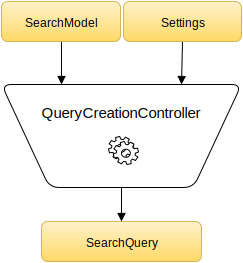
\includegraphics[width=0.4\textwidth]{QueryCreation}
  	\caption{Aufbau des Moduls QueryCreation}
	\label{fig:Aufbau des Moduls QueryCreation}
\end{figure}

QueryCreation generiert aus den Suchwörtern (SearchModel) und den Geräte- und App-Einstellungen ein allgemeines Anfrageformat. Diese Anfrageformat wird in QueryResolution zu einem für jede Suchmaschine spezifischen Suchformat umgewandelt.

\subsection{QueryCreationCtrl}

%\subsubsection{Unterteilabschnitt}
%\paragraph{Paragraph}
%\subparagraph{Unterparagraph}

\newpage
%\part{Konstruktion}
%\chapter{Programmlogik}

\section{SearchQuerys}
\newpage
%\part{Konstruktion}
%\chapter{Programmlogik}

\section{QueryResolution}

\subsection{JSONData}

\subsection{ResponseParse}
\subsubsection{FarooResponseParser}
\subsubsection{DuckDuckGoResponseParser}
\subsubsection{EexcessResponseParser}
\subsubsection{AbstractResponseParser}

\subsection{QuerySend}
\subsubsection{AbstractConnectionCtrl}
\subsubsection{JsonConnectionCtrl}
\subsubsection{URLConnectionCtrl}

\subsection{QueryProcessing}
\subsubsection{AbstractBuilder}
\subsubsection{AbstractJSONBuilder}
\subsubsection{AbstractURLBuilder}
\subsubsection{EexcessJSONBuilder}
\subsubsection{FarooURLBuilder}
\subsubsection{DuckDuckGoURLBuilder}
\subsubsection{EEXCESSOrigin}

%\paragraph{Paragraph}
%\subparagraph{Unterparagraph}

\newpage
%\part{Konstruktion}
%\chapter{Programmlogik}

\section{SearchResults}

SEARCHResults ist ein Container, welcher für ein Suchwort die Suchergebnisse speichert.
Der Container ist in der Lage, bei fehlenden Suchergebnissen Suchanfragen abzuschicken und informiert mit dem observel, ob neue Suchergebnisse von der Suchmaschine gekommen sind.
%\subsection{Teilabschnitt}
%\subsubsection{Unterteilabschnitt}
%\paragraph{Paragraph}
%\subparagraph{Unterparagraph}

\newpage
%\part{Konstruktion}
%\chapter{Programmlogik}

\section{Ranking}

\begin{figure}[ht]
	\centering
	\includegraphics[width=\textwidth]{Ranking}
	\caption{Ablauf des Rankings}
\end{figure}

Das Ranking dient der Sortierung der Suchergebnisse nach den Vorlieben des Nutzers. Das Sortieren der Zusatzinformationen wird durchgeführt, bevor die Ergebnisse dem Nutzer präsentiert werden. Das bedeutet, das Sortieren wird in der Klasse \lstinline|SearchResults| initialisiert und gestartet, nachdem die Zusatzinformationen aus dem Internet heruntergeladen wurden.

Die zur Zeit drei Persistency-Klassen \lstinline|PersistenceController|, \lstinline|RankingDataObject| und \lstinline|RankingDataObjectPersistency| werden im aktuellen Stand des Projektes noch nicht verwendet. Im weiteren Verlauf sollen die Klassen für das Speichern von nutzerspezifischen Informationen verwendet werden, um so die Suchergebnisse noch besser auf die Interessen des Nutzers zuschneiden zu können.

\pagebreak
\clearpage

Die Funktionalität des Rankings wird mit Hilfe von aktuell drei verschiedenen Regeln realisiert:

\begin{itemize}
	\item Language
	\item Mendeley
	\item MediaType
\end{itemize}

Jede dieser Regeln besitzt einen Faktor für die Gewichtung. Dieser legt fest, wie wichtig eine Regel ist. Für jeden Datensatz werden die oben genannten Regeln mit den entsprechenden Eingangsparametern erzeugt. Im weiteren Fortschritt des Projekts soll das Ranking dahingehend erweitert werden, dass nicht für jeden Datensatz alle Regeln erzeugt werden, sondern nur diejenigen, die für den jeweiligen Datensatz notwendig sind. So wird zum Beispiel für einen Datensatz, der nicht von der Suchmaschine Mendeley kommt, auch nicht die Regel \glqq Mendeley\grqq\xspace erzeugt. 

Die erstellten Regeln pro Datensatz werden in einem Hilfsarray zwischengespeichert (\lstinline|SearchRules|). Der Hauptteil des Rankings beginnt erst mit der Berechnung. Trifft eine Regel zu, also wenn der erwartete Wert der jeweiligen Regel dem tatsächlichen Wert des Suchergebnisses entspricht, so wird eine 1 (wahr) von der Regel zurückgeliefert. Trifft eine Regel nicht zu, so wird eine 0 (nicht wahr) zurückgeliefert. Die Rückgabewerte werden mit Hilfe des Enums \lstinline|RuleMatch| realisiert. Dieser Wert wird mit der Gewichtung der jeweiligen Regel multipliziert. Im Anschluss werden alle Ergebnisse aller Regeln, die zu einem Datensatz gehören, aufsummiert und durch die Anzahl der verwendeten Regeln dividiert. Dieser errechnete Wert gibt im Verhältnis wieder, in wie weit das Suchergebnis für den Nutzer interessant sein könnte. Nach dem Endergebnis werden alle Suchergebnisse zugehörig zu einem \SEARCH-Link absteigend nach diesem Wert sortiert und im Anschluss wieder dem Aufrufer zurückgegeben, der sie dann dem Nutzer präsentiert.
\newpage
%\part{Konstruktion}
%\chapter{Programmlogik}

\section{SettingsModel}
Im SettingsModel werden die verschiedenen Einstellungen für den Browser gespeichert.
Der Nutzer kann diese über das Einstellungsmenü des Geräts ändern.

\paragraph{Einstellungen}
Die Einstellugen sind in drei verschiedene Kategorien eingeteilt.
\begin{enumerate}  
     \item Suchmaschinen  
     \item Nutzerprofil
     \item Browsereinstellungen
\end{enumerate}

\subparagraph{Suchmaschinen}
Hier kann der Nutzer die verschiedenen Suchmaschinen einstellen, die für die SearchTags verwendet werden sollen.
Dabei kann entweder jede Suchmaschine einzeln gewählt werden, oder den Empfehlungen des Autors gefolgt werden.
Zur Auswahl stehen:
\begin{enumerate}  
     \item DuckDuckGo
     \item Eexcess
     \item Faroo  
\end{enumerate}
Sobald eine Suchmaschine gewählt wurde, werden die Empfehlungen des Autors ignoriert.

\subparagraph{Nutzerprofil}
Hier können die Nutzerdaten angegeben werden.
Davon wird bisher nur die Sprach verwendet.
Einstellungsmöglichkeiten:
\begin{enumerate}  
     \item Name  
     \item Alter  
     \item Stadt
     \item Land
     \item Sprache
\end{enumerate}

\subparagraph{Startseite}
Hier kann die Startseite des Browser festgelegt werden.



\listoffigures

\end{document}
